\section{Impulse response and frequency response}
\subsection{Recursive filters with a single pole\\}
Pole-zero plots of the single pole transfer functions with poles \(\gamma_1=0.3\),\(\gamma_1=0.95\),\(\gamma_1=1.05\) and \(\gamma_1=-0.95\) are found in figure~\ref{fig:1.1.zplane}.
Impulse responses are found in figure~\ref{fig:1.1.impz} and frequency reponses in figure~\ref{fig:1.1.freqz}.
\begin{figure}
	\center
	\includegraphics{./picture/ha6_1_1_zplane.eps}
	\caption{Pole-zero plots in the zplane of the transfer functions with the given poles. We note that \(\gamma_1=1.05\) results in an unstable system since it lies outside the unit circle.}
	\label{fig:1.1.zplane}
\end{figure}

\begin{figure}
	\center
	\includegraphics{./picture/ha6_1_1_impz.eps}
	\caption{Impulse responses of the given transfer functions. Points on the graph between samples do not contain meaningful values, but a stem plot makes it hard to see what is going on. Most of impulse response corresponding to the unstable system is not shown as it grows exponentially forever. Note that the blue line actually continues forever, but MATLAB does not provide points after the impulse response converges close to zero.}
	\label{fig:1.1.impz}
\end{figure}

\begin{figure}
	\center
	\includegraphics{./picture/ha6_1_1_freqz.eps}
	\caption{Frequency responses of the given transfer functions. Poles mirrored across the imaginary axis in the z-plane produce a phase response mirrored horizontally and vertically around the center axes and a magnitude response vertically mirrored around the normalized frequency of 0.5. This mirroring is the result of only plotting half of the frequency spectrum, in reality it is a horizontal translation. It can also be seen that poles in the negative half plane produce high pass filters and poles in the positive plane produce low pass filters. }
	\label{fig:1.1.freqz}
\end{figure}

\subsection{Recursive filters with double poles\\}
Pole-zero plots of the single pole transfer functions with double poles \(\gamma_{1,2}=0.3\),\(\gamma_{1,2}=0.95\),\(\gamma_{1,2}=1.05\) and \(\gamma_{1,2}=-0.95\) are found in figure~\ref{fig:1.2.zplane}.
Impulse responses are found in figure~\ref{fig:1.2.impz} and frequency reponses in figure~\ref{fig:1.2.freqz}.
The expectation is that these filters will have the same, but magnified, characteristics as their single pole counterparts.

\begin{figure}
	\center
	\includegraphics{./picture/ha6_1_2_zplane.eps}
	\caption{Pole-zero plot of the transfer functions in the z-plane. \(\gamma_{1,2}=1.05\) results in an unstable system}
	\label{fig:1.2.zplane}
\end{figure}

\begin{figure}
	\center
	\includegraphics{./picture/ha6_1_2_impz.eps}
	\caption{Impulse responses. It is interesting to note that while the transfer function with a pole pair at \(\gamma=0.3\) appears relatively unchanged, the poles closer to the unit circle result in a reponse value that initially grows before decaying as in the single pole case. The unstable filter does not have a meaningful impulse response.}
	\label{fig:1.2.impz}
\end{figure}

\begin{figure}
	\center
	\includegraphics{./picture/ha6_1_2_freqz.eps}
	\caption{Frequency responses. As expected these look identical to those in figure~\ref{fig:1.1.freqz} except for the change in scale.}
	\label{fig:1.2.freqz}
\end{figure}

\subsection{Recursive filters with complex conjugate poles}
Pole-zero plots of the single pole transfer functions with the conjugate poles \(\gamma_{1,2}=0.75\pm0.4i\),\(\gamma_{1,2}=0.75\pm0.75i\) and \(\gamma_{1,2}=-0.75\pm0.4i\) are found in figure~\ref{fig:1.3.zplane}.
Impulse responses are found in figure~\ref{fig:1.3.impz} and frequency reponses in figure~\ref{fig:1.3.freqz}.
We now expect to see more complex response dynamics in the form on oscillating impulse responses and resonance peaks in the frequency response.

\begin{figure}
	\center
	\includegraphics{./picture/ha6_1_3_zplane.eps}
	\caption{Pole-zero plots in the zplane of the transfer functions. The pole pair\(\gamma_{1,2}=0.75\pm0.75i\) is unstable as it is outside the unit circle.}
	\label{fig:1.3.zplane}
\end{figure}

\begin{figure}
	\center
	\includegraphics{./picture/ha6_1_3_impz.eps}
	\caption{Impulse responses. We see decaying oscillations for the stable filters and an exponentially growing oscillation from the unstable filter.}
	\label{fig:1.3.impz}
\end{figure}

\begin{figure}
	\center
	\includegraphics{./picture/ha6_1_3_freqz.eps}
	\caption{Frequency responses. We see the predicted resonance peaks in the magnitude response and the mirroring of poles mirrored acrossthe imaginary axis in the z-plane. The filters with conjugate poles in the right half plane now produce low frequency bandpass filters while the ones in the left half plane produce high frequency bandpass filters.}
	\label{fig:1.3.freqz}
\end{figure}

\subsection{Varying pole placement in the z-plane}
The magnitude of the given conjugate pole pair is \(C=\sqrt{0.75^2+0.75^2}=1.06\) and the angle is \(\Theta = \arctan(0.75/0.75) = \arctan(1) = 45^\circ\). Varying the angle or the magnitude changes both the phase and magnitude response of the filter.
This is because changing the magnitude of a pole moves it closer or further from the frequency circle and changing the angle moves the poles in relation to each other which changes their combined effect at the frequency circle. We will be examining both effects by looking
at filters with poles: \(\gamma_{1,2}=0.99e^{\pm i45^\circ}\),\(\gamma_{1,2}=0.74e^{\pm i45^\circ}\),\(\gamma_{1,2}=0.50e^{\pm i45^\circ}\),\(\gamma_{1,2}=0.25e^{\pm i45^\circ}\),\(\gamma_{1,2}=0.74e^{\pm i15^\circ}\),\(\gamma_{1,2}=0.74e^{\pm i75^\circ}\).

Pole-zero plots are found in figure~\ref{fig:1.4.zplane}, impulse responses and frequency responses in figure~\ref{fig:1.4.impz} and~\ref{fig:1.4.freqz}

\begin{figure}
	\center
	\includegraphics{./picture/ha6_1_4_zplane.eps}
	\caption{Pole-zero plots of the transfer functions. This time they are all stable.}
	\label{fig:1.4.zplane}
\end{figure}

\begin{figure}
	\center
	\includegraphics{./picture/ha6_1_4_impz.eps}
	\caption{Impulse responses. For the filters having poles with 45 degree angles, the oscillations decay fairly quickly and the amplitud is dependant on the magnitude of the pole. The poles with 75 and 15 degree angles both oscillate, but the 15 degree pole pair produces a rapidly decaying response as it is close to the real axis, while the 75 degree pole pair decays extremely slowly as it is close to the imaginary axis.}
	\label{fig:1.4.impz}
\end{figure}

\begin{figure}
	\center
	\includegraphics{./picture/ha6_1_4_freqz.eps}
	\caption{Frequency responses. Here we can see the sharp peak caused by the poles close to the frequency circle, this placement also causes the very sharp change in phase. It can also be seen that the decrease in amplitude from changing angles between 15 and 45 degrees is larger than the difference from 45 to 75. Furthermore, the poles with a magnitude smaller than 0.5 do not show a resonance peak and they pass most of the low frequencies with equal strength.}
	\label{fig:1.4.freqz}
\end{figure}

\subsection{Placing zeros}
Here we compare the complex conjugate pole pair \(\gamma_{1,2}=0.75\pm0.4i\) to the complex conjugate zero pair of the same value. 
Since a poles and zeroes have opposite effects on the transfer function, their frequency responses should be the same, but inverted.

The impulse responses, however, should be radically different since the filter containing only zeroes which makes it a finite impulse response filter while the filter with only poles will have an infinite impulse response.

Pole-zero plots are found in figure~\ref{fig:1.5.zplane}, impulse responses and frequency responses in figure~\ref{fig:1.5.impz} and~\ref{fig:1.5.freqz}

\begin{figure}
	\center
	\includegraphics{./picture/ha6_1_5_zplane.eps}
	\caption{Pole-zero plots in the zplane of the transfer functions.}
	\label{fig:1.5.zplane}
\end{figure}

\begin{figure}
	\center
	\includegraphics{./picture/ha6_1_5_impz.eps}
	\caption{Impulse responses. The finite nature of pole-less filter is clearly shown here.}
	\label{fig:1.5.impz}
\end{figure}

\begin{figure}
	\center
	\includegraphics{./picture/ha6_1_5_freqz.eps}
	\caption{Frequency responses. As expected they are each others opposites. Poles in the right half plane result in a lowpass filter while zeros in the right half plane result in a highpass filter.}
	\label{fig:1.5.freqz}
\end{figure}

